\section{Introduction}
\label{gwtf_sec:introduction}

\begin{figure}[t]
\centering
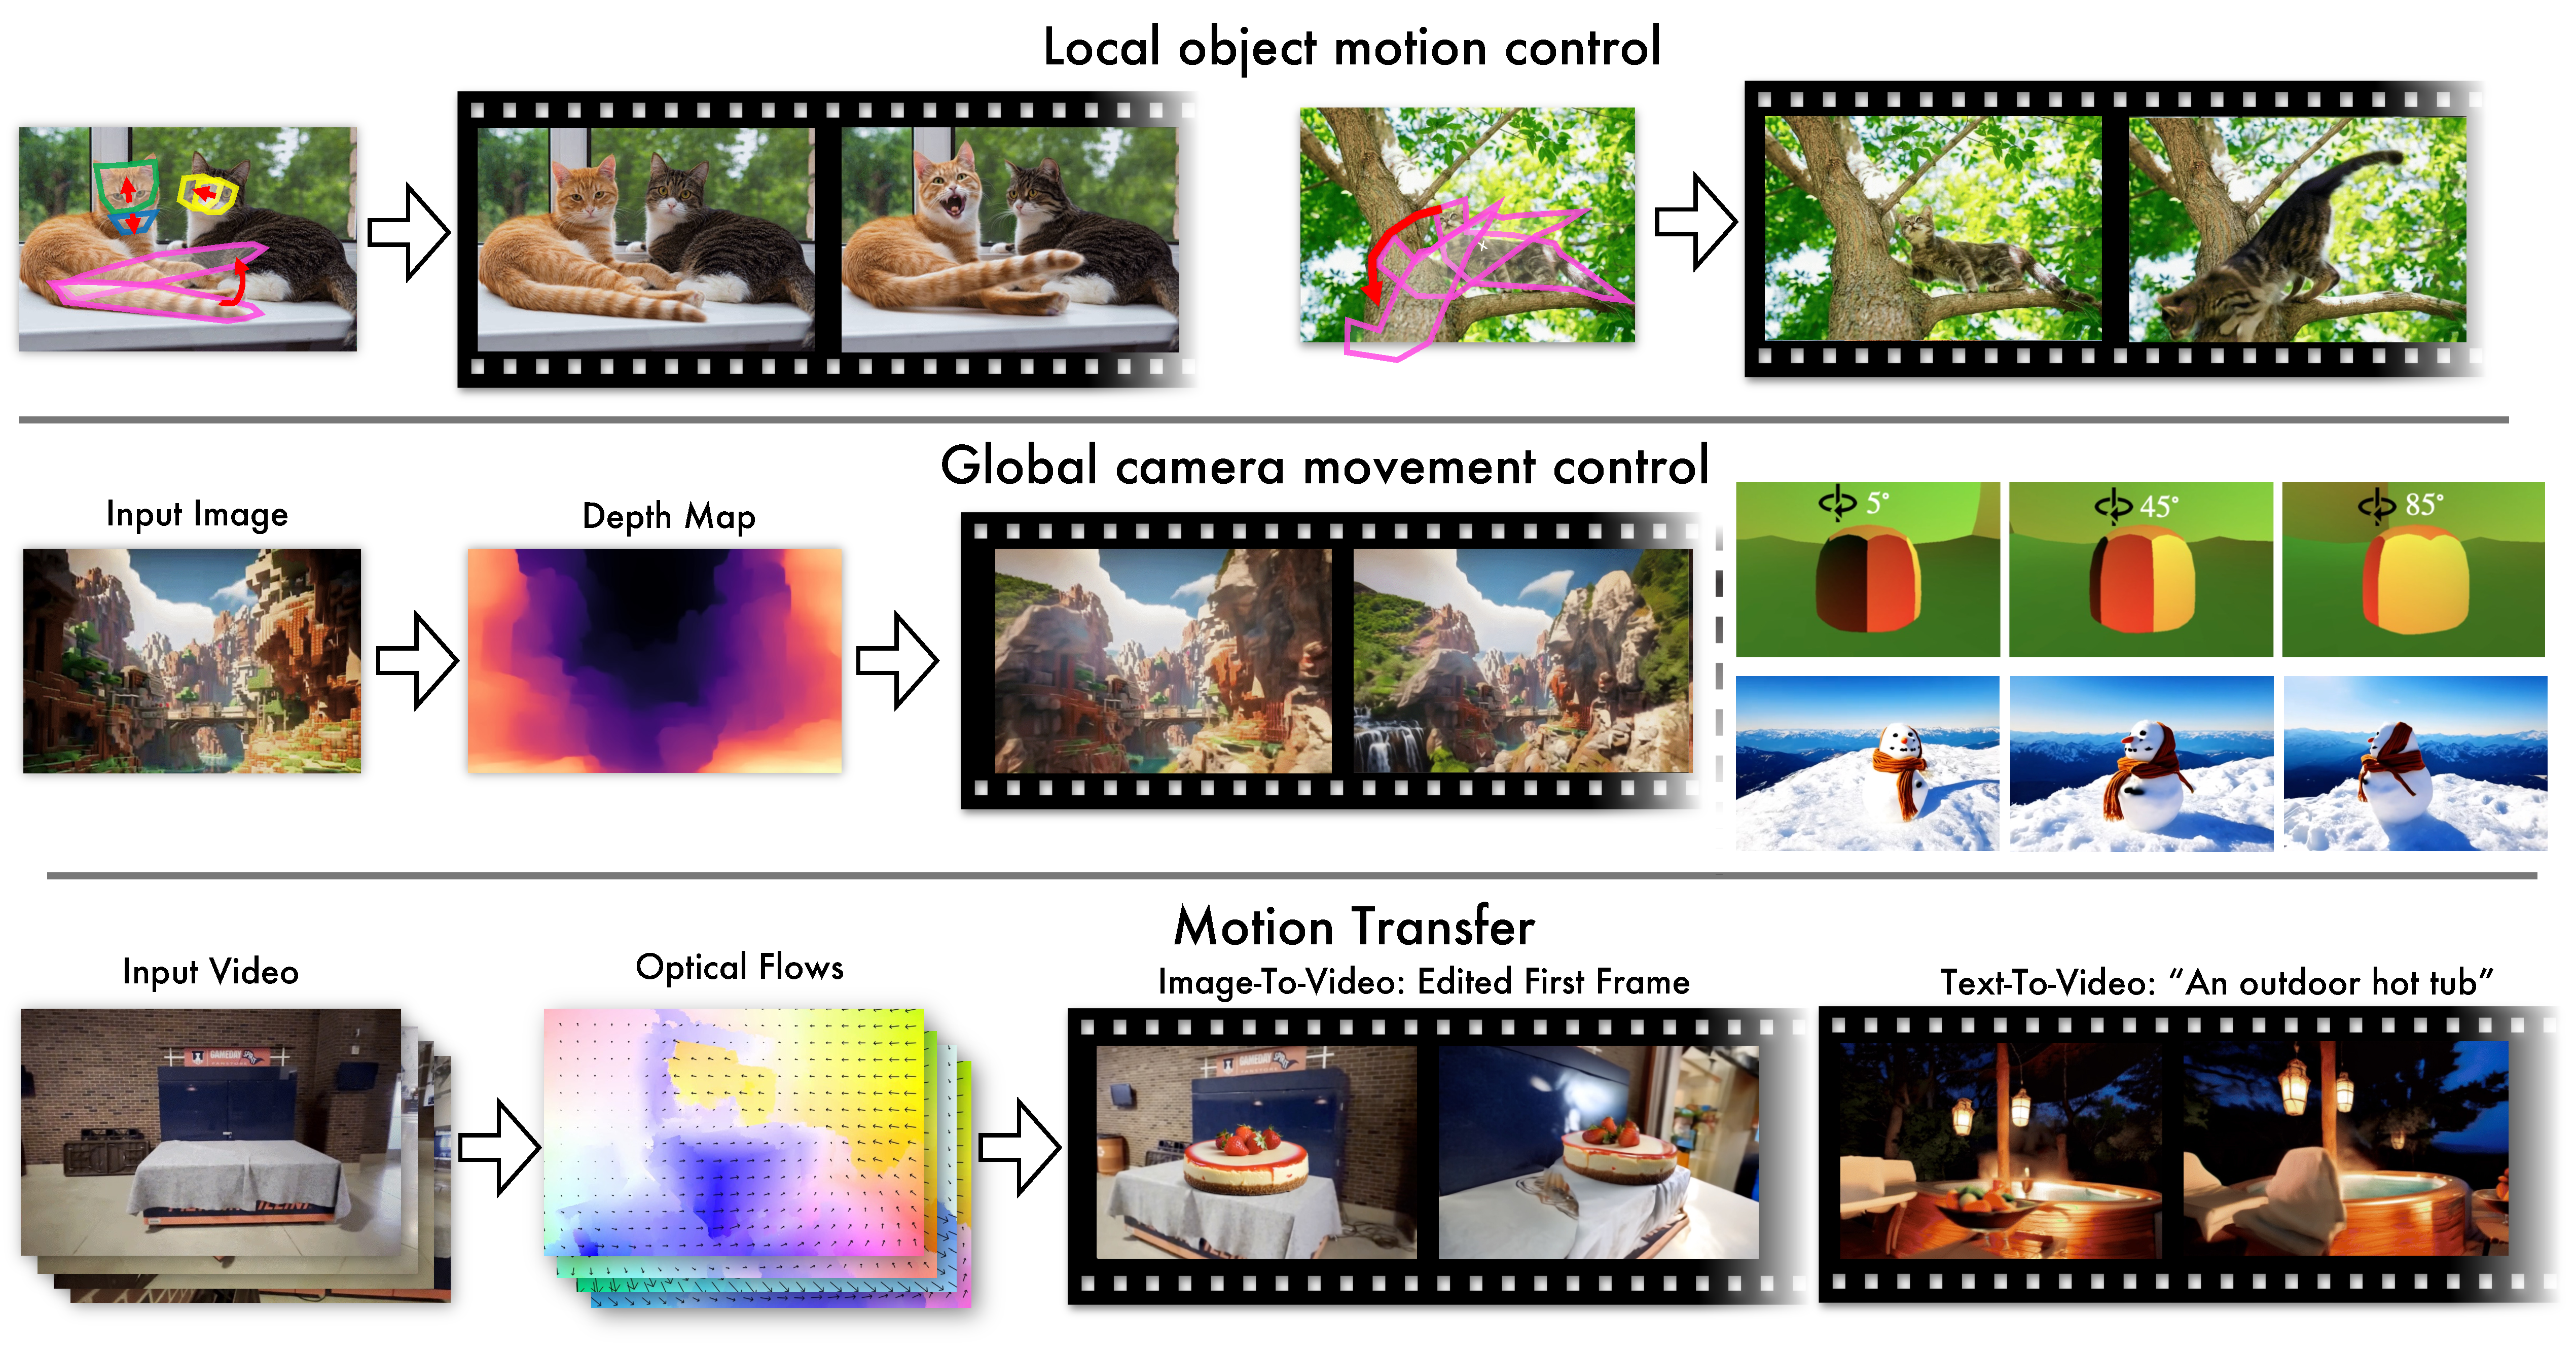
\includegraphics[width=\linewidth]{src/4_GWTF/fig/Teaser.pdf}
\caption[Go-with-the-Flow Overview]{Go-with-the-Flow presents a simple, robust, and easy-to-implement method for motion-controllable video diffusion models based on optical flow and noise warping. It only requires fine-tuning video diffusion models as a black box using warped noise patterns. Leveraging our models, we can (1) control the motion of individual objects or parts of those objects, (2) direct the camera movement by providing global flow fields corresponding to the desired movements, and (3) transfer the motion from input videos to target contexts.}
\label{gwtf_fig:teaser}
\end{figure}

\begin{figure}
    \centering
    \includegraphics[width=\linewidth]{src/4_GWTF/fig/framework_diagram.png}
    \caption[Go-with-the-Flow Framework Diagram]{Our method consists of three components: flow field extraction, real-time noise warping, and diffusion model fine-tuning/inference. During fine-tuning, we use the original captions of video samples. At inference, our method enables adaptation of reference motion to various prompts and/or initial frames, offering creativity and diversity in generation.
    }
    \label{gwtf_fig:framework_diagram}
\end{figure}

\begin{quote}
    "\textit{We adore chaos because we love to produce order.}" --- M. C. Escher, Dutch artist
\end{quote}

The essence of generative modeling lies in producing order from chaos, learning to transform random noise from the latent space into structured outputs that align with the distribution of training data. In this paper, we propose a novel approach to enhance generative model learning by proactively introducing partial order into the chaos of latent space sampling.

Our work is motivated by the remarkable progress in video diffusion generative models~\cite{guo2024animatediff,blattmann2023align,guo2024sparsectrl,blattmann2023stable,brooks2024video,yang2024cogvideox} and the equally significant challenges they face in terms of controllability beyond text and image guidance. Fine-grained interactive control over motion dynamics remains an under-explored area due to the intricate spatiotemporal correlations among video frames. The complexity of modern video diffusion architectures~\cite{brooks2024video,yang2024cogvideox}, which leverage 3D autoencoders~\cite{yu2024language} and spatiotemporal tokenizers~\cite{ma2024latte}, further complicates efforts to adapt models for effective motion control. The optimal format for defining and disentangling motion control from other guidance remains an open question.

Within the domain of motion-controllable video diffusion models, current applications typically fall into three categories: (1) local object motion control, represented by object bounding boxes or masks with motion trajectories~\cite{jain2024peekaboo,yang2024direct,wang2024motionctrl,shi2024motion,wu2024draganything,namekata2024sg,qiu2024freetraj,geng2024motion}; (2) global camera movement control, parameterized by camera poses and trajectories~\cite{yang2024direct,he2024cameractrl,kuang2024collaborative,wang2024motionctrl,xu2024camco,wu2024cat4d} or categorized by common directional patterns such as panning and tilting~\cite{guo2024animatediff,yang2024direct}; and (3) motion transfer from reference videos to target contexts specified by prompts or initial frames~\cite{wang2024videocomposer,yatim2024space,geyer2023tokenflow,yin2024scalable,ku2024anyv2v,ling2024motionclone,mou2024revideo,aira2024motioncraft}. However, these approaches share three key limitations: (1) they often necessitate complex modifications to the base model design such as guidance attention~\cite{qiu2024freetraj}, limiting compatibility with modern full-attention architectures involving spatiotemporal tokens~\cite{yang2024cogvideox}; (2) they are constrained to specific applications, requiring detailed parameterized motion signals, such as camera parameters, which are challenging to acquire or estimate accurately~\cite{zhang2024monst3r}, thus restricting generalizability across diverse scenarios; and (3) they are over-rigid to motion control at the cost of spatiotemporal visual quality.

To address these limitations, we propose a novel and straightforward method to incorporate motion control as a structured component within the chaos of video diffusion's latent space. We achieve this by correlating the temporal distribution of latent noise. Specifically, starting with a 2D Gaussian noise slice, we temporally concatenate it with warped noise slices, given the optical flow field~\cite{teed2020raft} extracted from a training video sample. \cref{gwtf_fig:framework_diagram} illustrates the diagram of our method. Our approach requires only a change in data: we pre-process training videos to yield warped noise and then fine-tune a video diffusion model. As it occurs solely during noise sampling, our method is agnostic to diffusion model design, requiring no modifications to model architectures or training pipelines. Surprisingly, removing temporal Gaussianity from the noise distribution does not deteriorate model fine-tuning. Instead, it can be quickly adapted after fine-tuning because temporal structure in the chaos of latent space facilitates generative learning and enables motion correspondence. Temporal coherence occurring in the latent space also harmonizes motion control with per-frame pixel quality by inheriting the high-quality prior from the base model.

It is worth noting that video diffusion fine-tuning relies on efficient noise warping algorithms that introduce minimal overhead during data pre-processing and noise sampling. The existing noise warping algorithm, \textit{How I Warped Your Noise} (HIWYN)~\cite{chang2024warped}, that maintains spatial Gaussianity and enables temporal flow warping, however, suffers from the quadratic computation costs w.r.t. frame count, making it much slower than in real time and therefore impractical for large-scale video diffusion model training. To address this, we propose a novel noise warping algorithm that runs fast enough in real time. Rather than warping each frame through a chain of operations from the initial frame, our algorithm iteratively warps noise between consecutive frames. This is achieved by carefully tracking the noise and the flow density along a forward and a backward flow at the pixel level, accounting for both expansion and contraction dynamics, supplemented with conditional white noise sampling from HIWYN~\citet{chang2024warped} to preserve Gaussianity. \cref{gwtf_alg:main} provides further details. We validate the spatial Gaussianity and time complexity of our noise-warping algorithm and apply it to training-free image diffusion models for quantitative and qualitative assessments of controllability and temporal consistency.

During video diffusion inference, our method offers a one-stop solution for diverse motion control applications by adapting noise warping based on motion type. (1) For local object motion, we interactively transform noise elements within object masks given users' dragging signals. (2) For global camera movement control, we reuse the optical flows from reference videos to warp input noise, and regenerate videos conditioned on different texts or initial frames. (3) For arbitrary motion transfer, the motion representations are not limited to optical flows~\cite{teed2020raft}, but also include flows from 3D rendering engines~\cite{villar2021learning}, depth warping~\cite{yu2024wonderjourney}, etc. We validate the effectiveness of our solution across various video generation tasks, demonstrating its ability to preserve consistent motion across different contexts or render distinct motions for the same context. Extensive experiments and user studies indicate the advantages of our solution in pixel quality, motion control, text alignment, temporal consistency, and user preference.

In summary, our contributions include:

(1) A novel and simple one-stop solution for motion-controllable video diffusion models, integrating motion control as a flow field for noise warping in latent space sampling, plug-and-play for any video diffusion base models as a black box, and compatible with any other types of controls.

(2) An efficient noise warping algorithm that maintains spatial Gaussianity and follows temporal motion flows across frames, facilitating motion-controllable video diffusion model fine-tuning with minimal overhead.

(3) Comprehensive experiments and user studies demonstrating the overall advantageous pixel quality, controllability, temporal consistency, and subjective preference of our method on diverse motion control applications, including but not limited to: local object motion control, motion transfer to new contexts, and reference-based global camera movement control.
